\setcounter{chapter}{5}
\setchapterabstract{This chapter addresses EU merger remedies, which are modifications proposed by parties to resolve competition concerns identified by the European Commission, allowing conditional clearance of mergers. Remedies aim to eliminate competition concerns, be easily implementable, and ensure lasting market effectiveness without creating new competition issues. Structural remedies involve divestiture or severing links to competitors, enabling market competition through viable stand-alone businesses or asset packages. Buyers of divested assets must be independent, financially capable, and incentivized to sustain competitiveness. Behavioural remedies, less favoured, impose commitments on future conduct but require burdensome monitoring and long-term enforcement. The remedy process includes market tests, consulting third parties like competitors and customers, to evaluate suitability and effectiveness. However, third-party interests can sometimes lead to overreaching remedies. Breaches of remedies lead to revocation of clearance, fines, or dissolution orders, ensuring compliance with EU competition standards.}
\chapter{Merger Remedies}
\vspace{-1.5cm}

\setcounter{chapter}{16}
{\chaptoc\noindent\begin{minipage}[inner sep=0,outer sep=0]{0.9\linewidth}\section*{Introduction: the EU System}\end{minipage}}

If the EU Commission finds out that a merger creates a significant impediment to effective competition in the relevant market(s), it can prohibit the transaction from being implemented or clear it subject to remedies (that must fully resolve the competition concerns).

Remedies consist in:
\begin{itemize}
    \item A modification to a concentration that is...
    \item offered by the Parties, either in Phase I or in Phase II, with the aim...
    \item to resolve the competition concerns identified by the Commission, and
    \item thereby allowing clearance of the transaction (subject to the remedy).
\end{itemize}

As of 31 October 2024, out of 9431 notifications, the Commission approved mergers subject to conditions and obligations:
\begin{itemize}
    \item 357 in Phase I
    \item 151 in Phase II (i.e.: $>$ 50\% of the 255 Phase II decisions taken to date)
\end{itemize}

\newpage
\subsection*{Allocation of Responsibilities}

    \begin{figure}[ht]
        \centering
        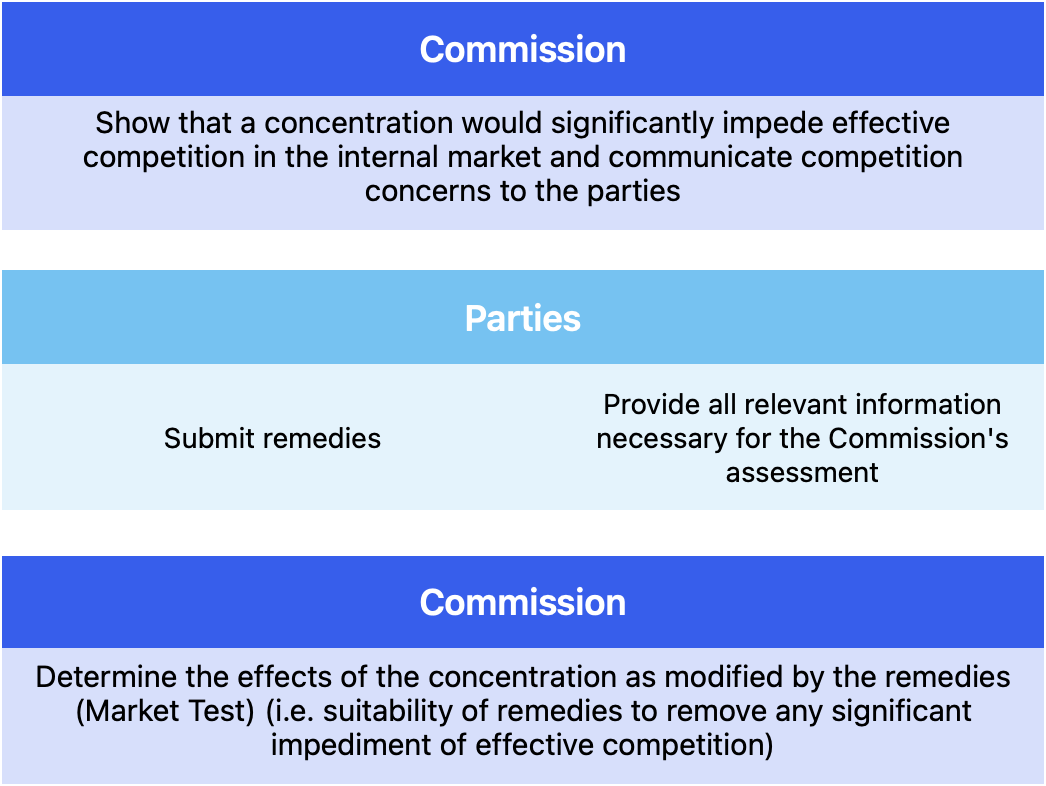
\includegraphics[width=0.75\linewidth]{graphics/L16-1.png}
    \end{figure}

\section{General principles}

The type of remedy suitable to eliminate competition concerns is determined on a case-by-case basis.

        \subsubsection{Public Perspective}

            Acceptable remedies should:
            \begin{itemize}
                \item Eliminate competition concerns entirely;
                \item Be capable of being implemented easily and effectively
                within a short period of time.
            \end{itemize}
            
            Remedies cannot be too extensive and complex, making it impossible to determine with certainty, at the time of the decision, that they will be fully implemented and are very likely to maintain effective competition in the market:
            \begin{itemize}
                \item Represent a permanent solution and do not raise any different competition concern.
            \end{itemize}

        \subsubsection{Private Perspective}

            To protect private parties, remedies \textbf{MUST BE} proportionate. The
            Commission:
            \begin{itemize}
                \item shouldn’t seek remedies going beyond what is required to resolve the competition concerns;
                \item has no power to impose obligations on third parties, only on the notifying parties;
                \item Must take into account the benefits of the transaction for consumers in assessing proposed commitments. In particular, the Commission prefers remedies that capture such benefits to those that do not.
            \end{itemize}

\section{Structural or Behavioural}

    \subsubsection{Structural Remedies}

    Structural remedies cause an immediate change in the structure of the relevant market:
    \begin{itemize}
        \item divestment of a market position through the disposal of assets, shares, patents, trademarks or IP rights; the termination of exclusive distribution agreements; severance of links with suppliers, customers or competitors.
    \end{itemize}
    
    Some remedies are categorized as \textquotedblleft quasi-structural\textquotedblright{} if they have a structural effect on the market (i.e., facilitate new entry or prevent foreclosure) without amounting to a divestiture:
    \begin{itemize}
        \item access remedies allow third parties to access key infrastructures, networks, technologies including patents on a fair, reasonable, non-discriminatory (FRAND) and transparent basis.
    \end{itemize}
    
    There is a strong preference for structural remedies as they are seen to be easier to implement and do not require medium or long-term monitoring.

    \subsubsection{Behavioural Remedies}
    
    Behavioural remedies involve a commitment by the merging parties to act (or to refrain from acting) in a certain manner in the future:
    \begin{itemize}
        \item granting access to products on equal terms; maintain a certain price, do not increase prices over the inflation rate, duty to supply, etc.
        \item They cannot consist in a commitment not to violate competition law (e.g., from now on, I will not abuse my dominant position again), but can consist in obligations not to adopt a particular strategy (e.g., tying and bundling) if that is the Commission’s theory of competitive harm.
        \item Usually they involve complex long-term (time-consuming and burdensome) monitoring and reporting obligations; it may cause further litigation on the fulfilment of the various conditions/commitments (between the parties or vis-à-vis the Commission).
    \end{itemize}
    
    \Remark{
    Behavioural remedies are accepted if they are as effective as a divestiture.
    }

    \subsection{Structural Remedies}

        \subsubsection{Divestment}

            (short of prohibition) The most effective way to ensure that a merger does not significantly impede effective competition is:
            \begin{itemize}
                \item Creating the conditions for the emergence of a new competitor\sn{\Example{
            When the mobile operators “3” and “Wind” merged they had to divest some business – antennas, etc. - in favour of a new entrant competitor, Iliad.
            }}, or
            
                \item Strengthening existing (weaker) competitors.
            \end{itemize}

\newpage
        \subsubsection{Divestment Procedure}

            Can be achieved via full or partial divestiture of a market position by the parties:
            \begin{itemize}
                \item Stand-alone business: viable business that can operate independently of the merging parties and compete effectively on a lasting basis (e.g., pre-existing corporation/company, business division, plant, etc.).
                \item Carve-out: package of assets part of an existing business that is retained by the parties.
            \end{itemize}

            \Remark{
            The Commission only accepts carve-outs if they consist in a viable stand-alone business once transferred to a suitable purchaser.
            }
            
            Or possibly with the removal of structural links with competitors, suppliers, or customers (if they raise competition concerns): e.g., divestment of the participation to a JV, divestment of minority shareholdings (and interlocking directorates), termination of long-term supply or distribution arrangements (if the transaction forecloses inputs for competitors upstream or access to customers downstream).

        \subsubsection{Divestment Business}

            Divestitures include all assets contributing to the current operation or that are necessary to ensure the viability and competitiveness of the divested business and all personnel currently employed by the divested business or which are necessary to maintain its viability and competitiveness. Vendor should not deprive the to-be-divested business of its value (and competitive relevance) before sale.

            Types of assets that can be divested (some or all together):
            \begin{itemize}
                \item \textbf{Tangible assets}: R\&D, production or distribution facilities, sales and marketing material.
                \item \textbf{Intangible assets}: e.g., trademarks, patents, know-how, client list.
                \begin{itemize}
                    \item The Commission may accept a divestiture package consisting of brands (and supporting manufacturing and distribution assets) where the resulting business will be viable in the hands of a suitable purchaser and trademarks are of vital importance in the sector in question and are one of the main factors in final consumers’ choices (for example clothing, fashion, beers...).
                \end{itemize}
                \item \textbf{Permits and authorizations} by public bodies.
                \item \textbf{Contracts, leases and arrangements} (supply, manufacturing, licensing, marketing, distribution, etc.).
                \item \textbf{Customer contracts}, lists, credits, records, transactional data and other records.
                \item \textbf{Personnel} (R\&D, manufacturing, sales...) essential for viability and competitiveness of the business.
            \end{itemize}

        \subsubsection{Who is the Buyer?}

        In addition to the viability of the business to divest, the parties have to persuade the Commission of the suitability of the proposed buyer.

        \begin{enumerate}[label=(\alph*)]
            \item The buyer must have the capabilities to continue the business as a viable competitor and particularly:
            \begin{itemize}
                \item Be independent of and unconnected to the parties (i.e., the merging parties must not be in the position to influence the acquirer’s behavior).
                \item Possess the financial resources, relevant expertise, incentive, and ability to maintain and develop the divested business as a viable and active competitive force in the market (based on a specific business plan).
            \end{itemize}
            Financial buyers (PE, Management LBOs) are not necessarily excluded, but they have to prove to have sufficient experience and capabilities in the market segments affected by the remedy and that the divestment business is truly stand-alone. There is, in any event, a risk of a broader remedy package.
            \item The divestiture transaction does not in itself raise significant competition concerns or risks of delayed implementation.
            \begin{itemize}
                \item Often, they require the buyer to be an out-of-area competitor or a viable actual competitor but with a market share lesser than X\%, etc.
            \end{itemize}
        \end{enumerate}

        \Remark{
        The Commission's role is to approve or disprove the proposed purchaser, not to select among or compare a range of potential purchasers. Once a divestiture is made a condition of the clearance decision, it is a matter for the parties to find a suitable purchaser for the business.
        }

        \Remark{
        The Buyer is normally identified only after the remedies have been accepted by the Commission and the transaction has been conditionally cleared (sometimes before).
        }

        \subsubsection{Procedure - Market Test}

            When offered a remedy, the Commission will consult on the proposed remedies with NCA and third parties (customers, suppliers, competitors) in the form of a market test.
            \begin{itemize}
                \item The Commission sends out a summary of the proposed remedies together with a questionnaire to specific undertakings.
                \item After responses have been received, the Commission often has calls or meetings with interested third parties to clarify their responses.
            \end{itemize}
            
            The Commission conducts market tests for almost all remedy proposals to determine whether proposed remedies sufficiently address competition concerns\sn{\Note{The Commission seeks opinions of third parties on:
            \begin{itemize}
                \item Workability, effectiveness, and suitability of the remedies to address competition concerns;
                \item Specific weak points to be improved;
                \item Viability and competitiveness of the divestment business;
                \item Potential interested buyers.
            \end{itemize}}}.
            
            There are concerns that the Commission places too much reliance on the outcome of the market test, which can be problematic as third parties often have an interest (or self-interest) and may manipulate the process. This may result in remedies going beyond what is strictly necessary to address the actual competition issues raised by the transaction.

\section{Breach of Remedies}

    The Commission makes a distinction between conditions and obligations.
    \begin{itemize}
        \item \textbf{Conditions:} actions required to achieve the structural change in the market (e.g., sale of the business unit).
        \item \textbf{Obligations:} implementing steps necessary to achieve the modifications sought (e.g., trustee appointment, viability and competitiveness, ring-fencing, hold-separate).
    \end{itemize}
    
    If a condition is not met:
    \begin{itemize}
        \item Clearance decision is no longer applicable;
        \item The concentration is deemed not authorized (the situation rendering the concentration compatible with the internal market didn’t materialize);
        \item The concentration is treated as if implemented without authorization;
        \item The Commission can take interim measures, order the parties to dissolve the concentration, and impose fines (up to 10\% of turnover).
    \end{itemize}
    
    If an obligation is not met:
    \begin{itemize}
        \item The Commission may revoke the clearance decision and impose fines; or
        \item It will require parties to cure the breach within a fixed deadline.
    \end{itemize}

    